\documentclass[12pt]{article}
\usepackage[margin=1in]{geometry}
\usepackage[usenames,dvipsnames]{xcolor}
\usepackage[T1]{fontenc}
\usepackage{fancyhdr}
\usepackage{listings}
\usepackage{graphicx}
\usepackage{hyperref}
\usepackage{mdframed}

\lhead{CpSc 210: Programming Methodology}
\chead{\empty}
\rhead{Fall 2015}
\lfoot{\empty}
\cfoot{\thepage}
\rfoot{\empty}

\definecolor{light-gray}{gray}{0.93}
\definecolor{text-gray}{gray}{0.22}

\lstset{
	basicstyle=\color{text-gray}\ttfamily,
	columns=fixed,
	fontadjust=true,
	basewidth=0.5em
}

\hypersetup{
	colorlinks=true,    
	urlcolor=RubineRed,
}

\color{text-gray}
\begin{document}
\title{\vspace{-.35in}Lab \#5: Singly-Linked List}
\date{\empty}
\maketitle

\pagestyle{fancy}
\thispagestyle{fancy}

\vspace{-.75in}
\section{Objectives}
In this lab you will be writing a bare-bones implementation of a singly linked list. When you're done with this lab, you should understand and be able to employ ``void'' pointers in your code, gain some familiarity with developing type-general, linked data-structures, and work more effectively with pointers in general.

\subsection{Downloading}

You can download your starter kit by following the instructions below:

\begin{itemize}
\item first, create a \texttt{lab4} directory under your existing cpsc 210 lab directory 
\item then type: \texttt{wget ...}
\item after this, decompress the file with \texttt{unzip lab5.zip}
\item finally, delete the packaged download by typing \texttt{rm lab5.zip}
\end{itemize}

These instructions should be pretty much routine to you at this point, and as such, will disappear from these handouts.

\section{Background: void pointers and type casting}

A \textit{void pointer} can be used to hold the address of an arbitrary data type. By way of example, consider the following code:

\begin{mdframed}[backgroundcolor=light-gray, innerleftmargin=10, innertopmargin=1,innerbottommargin=1,linecolor=light-gray]
\begin{lstlisting}
int x;
float y;

// declare a struct capable of being referenced as s_type --
// this is what the `typedef' part accomplishes
typedef struct s {
    int f1;
    int f2;
} s_type;

s_type s1, *sp;
void *p;
\end{lstlisting}
\end{mdframed}

\noindent The void pointer \texttt{p} can be set to point to any of the objects above, (e.g.: \texttt{p = \&x}, \texttt{p = \&y}, \texttt{p = \&s1}, etc). You can also write \texttt{p = sp} or \texttt{sp = p} without any problem since both \texttt{p} and \texttt{sp} are of type pointer; they just happen to be pointing to different types of objects. \\

\noindent However, we run into trouble when I attempt to use \texttt{p} to access a field. For example, if I write \texttt{x = *p} I get the following (helpful?) message from the compiler that reads something like:

\begin{mdframed}[backgroundcolor=light-gray, innerleftmargin=10, innertopmargin=1,innerbottommargin=1,linecolor=light-gray]
\begin{lstlisting}
warning: dereferencing `void *' pointer ... 
error: void value not ignored as it ought to be
\end{lstlisting}
\end{mdframed}

\noindent There are two ways to avoid this:
\begin{enumerate}

\item \textbf{type casting:} I can tell the compiler the type of the data that \texttt{p} is pointing to:
\begin{mdframed}[backgroundcolor=light-gray, innerleftmargin=10, innertopmargin=3,innerbottommargin=0,linecolor=light-gray]
\begin{lstlisting}
x = *(int *)p;
\end{lstlisting}
\end{mdframed}

\item \textbf{extra pointers:} The alternative is to simply define another pointer:
\begin{mdframed}[backgroundcolor=light-gray, innerleftmargin=10, innertopmargin=1,innerbottommargin=1,linecolor=light-gray]
\begin{lstlisting}
int *q;
...
q = p;
x = *q;
\end{lstlisting}
\end{mdframed}
Personally I find that defining a few extra pointers results in more readable code, and will likely be less error-prone (but either approach gets the job done -- so it's up to you).
\end{enumerate}

\section{An additional example}

Here's another example using the above structure. Assume we want to set the \texttt{f2} field in \texttt{s1} to an integer (say, 6), and suppose that \texttt{p} points to \texttt{s1}. At this point, based on the two approaches discussed above, we could write either:

\begin{mdframed}[backgroundcolor=light-gray, innerleftmargin=10, innertopmargin=1,innerbottommargin=1,linecolor=light-gray]
\begin{lstlisting}
((s_type *)p)->f1 = 6;     //approach #1
\end{lstlisting}
\end{mdframed}
\noindent or alternatively
\begin{mdframed}[backgroundcolor=light-gray, innerleftmargin=10, innertopmargin=1,innerbottommargin=1,linecolor=light-gray]
\begin{lstlisting}
sp = p;                // approach #2
sp->f1 = 6;
\end{lstlisting}
\end{mdframed}

\section{Task: list implementation}

In class \href{http://people.cs.clemson.edu/~rlowe/cs2100/notes/linked-list.pdf}{you've already seen} the implementation of a relatively simply linked-list data structure. In this lab you are going to alter what was discussed in two key respects, \textbf{so pay attention:}

\begin{itemize}
\item objects of \textit{arbitrary} type can now be stored in the list: meaning when you're done, your list will be able to hold \texttt{float}s, \texttt{char}s, or other custom, user-defined datatypes.
\item new additions to a list, rather than being appended to the \textbf{tail} (end), are instead to be added to the \textbf{head} (front).
\end{itemize}

\subsection{Key structures}

In \texttt{list.h} we provide two structures that give us everything we need to implement the desired list data structure. 

\subsubsection{\large{\texttt{node}}}

The first of these is \texttt{node}
\begin{mdframed}[backgroundcolor=light-gray, innerleftmargin=10, innertopmargin=1,innerbottommargin=1,linecolor=light-gray]
\begin{lstlisting}
typedef struct node_t {
   struct node_t *next;   // pointer to the next node
   void *data;         	  // the data pointed-to-by/stored at this node
} node;
\end{lstlisting}
\end{mdframed}

\noindent Think of a \texttt{node} as one link in a chain of \textit{n} nodes that form the backbone of our list. This particular struct consists of two fields:
\begin{itemize}
\item a \texttt{next} pointer that points to the next \texttt{node} in the chain, if there is indeed such a node; \texttt{null} otherwise
\item a void pointer called \texttt{data} that points to an arbitrarily-typed object (could be number, string, vector, tree, etc)
\end{itemize}

\noindent Given our definition of \texttt{node}, pictorially, a list of integers such as \texttt{[5, 2, 7]} would internally look something like:

\begin{center}
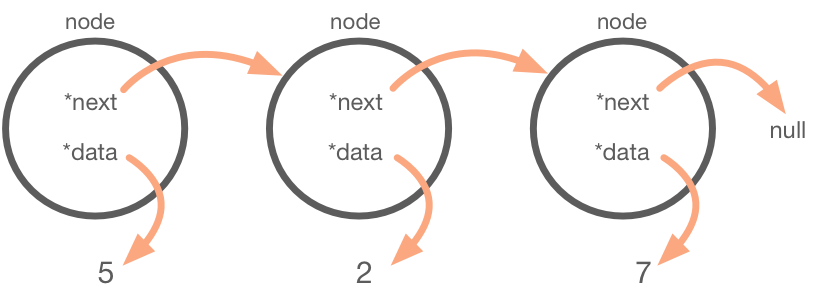
\includegraphics[scale=0.60]{figures/node_diag1.png}
\end{center}

\subsubsection{\large{\texttt{list}}}
The second and final piece of our implementation is the \texttt{list} struct:
\begin{mdframed}[backgroundcolor=light-gray, innerleftmargin=10, innertopmargin=1,innerbottommargin=1,linecolor=light-gray]
\begin{lstlisting}
typedef struct list_t {
   node_t *current;     // current list position 
   node_t *head;        // the head (starting node) of our list
} list;
\end{lstlisting}
\end{mdframed}

\noindent You can think of \texttt{list} as the manager, or controller, of an entire list. The \texttt{list} controller keeps track of two important pieces of information:
\begin{itemize}
\item a current position pointer that points to \textit{one} particular \texttt{node} within the list.
\item a \texttt{head} pointer which always points to the \texttt{node} at the \texttt{head} of the list; if the list is empty, \texttt{head == NULL}
\end{itemize}

\noindent So in terms of our previous \texttt{[5, 2, 7]} example, \texttt{list} adds the following to our illustration:

\begin{center}
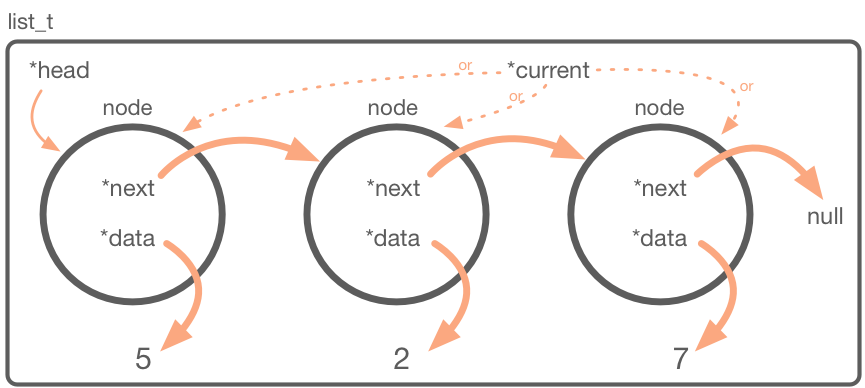
\includegraphics[scale=0.60]{figures/node_diag2.png}
\end{center}

\subsection{List functions}

Here are the prototypes for the list functions that you are expected to implement. 

\begin{mdframed}[backgroundcolor=light-gray, innerleftmargin=10, innertopmargin=1,innerbottommargin=1,linecolor=light-gray]
\begin{lstlisting}
/** Creates and returns a `new' list controller object. You'll need to 
 *  use C's malloc (`M'emory`ALLOC'cation) function.
 */
list *init();

/** Given an existing (possibly empty) list `l' and a pointer to a piece 
 *  of `data', this method creates a new node containing `data' and and 
 *  puts the new node on the front of `list'.
 */
void prepend(list *l, void *data);


/** Sets the current position pointer of list `l' to head. */
void reset(list *l);

/** Returns a pointer to the data field of the node pointed to by 
 *  `current' and advances the 'current' pointer to the next node.
 */
void *next(list *l);
\end{lstlisting}
\end{mdframed}

\section{Testing}

Assuming you are in the directory housing your code, to run all you need to do is type \texttt{make}. This will compile and generate an executable for your code named \texttt{lab5}. To run the generated executable, simply type \texttt{./lab5}. Additionally, typing \texttt{make clean} will freshen your current working directory by deleting any gcc-generated \texttt{*.o} files. \\

\noindent The \texttt{listtest.c} driver provided currently only prints the contents of \texttt{num\_list}. Your job is to extend the existing tests so that it prints out the contents of \texttt{fruit\_list} and \texttt{car\_list}. \\

\noindent Iterate and use your \texttt{next()} method to access and print the contents of the lists, formatting your output like so:

\begin{mdframed}[backgroundcolor=light-gray, innerleftmargin=10, innertopmargin=1,innerbottommargin=1,linecolor=light-gray]
\begin{lstlisting}
num_list: 25, 20, 15, 10, 5,
fruit_list: banana, peach, orange, apple,
car_list: [Toyota Camry 2010], [Honda Accord 2010], [Ford Mustang 2009],
\end{lstlisting}
\end{mdframed}

\section{Hints}

\begin{itemize}
\item When implementing \texttt{init()} remember to initialize current and head fields to \texttt{NULL}. If you don't do this, asking if some field of your list \texttt{== NULL} will likely not work (in all likelihood you'll get a segmentation fault).

\item There are two cases to deal with in the implementation of \texttt{prepend()}: one in which the list you're appending to is empty (how do we detect this?), and the more general case when the list already contains one or more elements.

\item When you \texttt{prepend()} an element to your list, \texttt{head} should be reassigned to point at the newly appended element, and \texttt{current} can as well. \textbf{Note:} if you don't reassign \texttt{current} in \texttt{prepend()},  you'll need to remember to call \texttt{reset()} before you try to print a list!
\end{itemize}

\section{Handin}

When you're finished, and you are confident your work is \textbf{adequately commented} and \textbf{correct}, go ahead and `tarify' with the following command:
\begin{center}
\texttt{tar cvf lab5\_handin.tar list.c list.h listtest.c MakeFile}
\end{center}
\noindent and submit the resulting \texttt{lab5\_handin.tar} to the appropriate bucket on handin.
\end{document}
